%!tex root=thesis.tex
\chapter{Machine Learning on Crowds}

\todo{Add a nice chapter summary.} In this chapter, I will introduce some
concepts from machine learning that I will use for the rest of this thesis. I
will discuss some common classification methods and techniques, describe image
feature extraction using convolutional neural networks, survey some methods to
combat label noise, and discuss the use of active learning to improve labelling
efficiency.

\section{Discuss some machine learning here}

\section{Crowdsourced Labelling}

    \section{Notation}

        \todo{add a notation section (maybe even not here)}

    \section{Crowdsourced Labels}
        
        For standard supervised learning tasks, the labels are generally
        provided by some \emph{expert}, carrying the assumption that these
        labels are correct and represent the groundtruth. More recently,
        however, many projects have
        \emph{crowdsourced} their labels: Non-expert people (the \emph{crowd})
        volunteer or are paid to label data. The most obvious advantage of
        crowdsourcing is that crowds are able to cheaply or quickly label large
        amounts of data simply because there are so many people labelling. The
        crowd may be sourced from websites like Amazon Mechanical
        Turk\footnote{\url{http://mturk.com}} where small amounts of money are
        paid on a per-label basis, or they may volunteer out of interest in the
        labelling project. Some notable examples of projects with crowdsourced
        labels include Galaxy Zoo \citep{lintott08}, a project to identify
        morphologies of galaxies from the Sloan Digital Sky Survey that has
        gathered tens of millions of labels for nearly 900 000 galaxies from
        over 80 000 volunteers
        \citep{lintott11}; and Snapshot Serengeti \citep{swanson15}, a project to
        observe mammals in Serengeti National Park that has classified nearly
        11 million camera trap images with the help of 28 000 volunteers.
        However, crowdsourcing is not without downsides. Since the crowd
        necessarily consists of non-experts, there is no longer any guarantee
        that labels are correct --- indeed, for the Radio Galaxy Zoo, balanced
        accuracy of individual labellers varies from 40--100\%, with an average
        of 71\%. Additionally, labels from different labellers may be
        correlated, different labellers may be better skilled at labelling
        different kinds of examples, some examples may be intrinsically hard
        for non-experts to label, and labellers may even be actively malicious
        in giving incorrect labels.

    \subsection{Majority Vote}

        One way to reduce label noise is to allow multiple labellers to label the same examples, and then for each example take the \emph{majority vote} to find a ``consensus'' label. If the label provided by the $t$th labeller is denoted $y_t$ and there are $T$ labellers, then the consensus label is given by
        \begin{equation*}
            y = \begin{cases}
                1 & \frac{1}{T} \sum_{t = 1}^T y_t > 0.5\\
                0 & \frac{1}{T} \sum_{t = 1}^T y_t < 0.5\\
            \end{cases}
        \end{equation*}
        with the remaining case decided evenly at random \citep{raykar10}.

        The idea is that the majority of labels are correct, so with sufficiently large amounts of relabelling we expect the label noise to be reduced. How large ``sufficiently large'' is is unclear and domain-dependent, and is outside the scope of this thesis, though papers like \citet{sheng08} and \citet{lin16} provide some information on how to choose relabelling rates. Of course, this fails in situations where the majority of labellers are not correct, which may be due to intrinsic difficulty or malicious labelling, or where there is no clear majority.

    \subsection{Modelling Labeller Reliability}

        In crowd learning scenarios, it is common to have multiple labels for a data point with no known groundtruth. One way to deal with this is to jointly model both the reliability of each labeller (the \emph{labeller model}) and the groundtruth itself (the \emph{classification model}). Methods following this approach are developed in \citet{raykar10} and \citet{yan10}. These methods make different assumptions on the labellers. I describe these methods in detail here.

        \subsubsection{Raykar et al. Method}
            \label{sec:raykar}

            \citet{raykar10} propose modelling the $t$th labeller by two parameters $\alpha_t$ and $\beta_t$. $\alpha_t$ is the \emph{sensitivity} and $\beta_t$ is the \emph{specificity} of labeller $t$, i.e.
            \begin{align*}
                \alpha_t &= p(y_t = 1 \mid z = 1)\\
                \beta_t &= p(y_t = 0 \mid z = 0).
            \end{align*}
            This model assumes that labeller reliability is independent of the example $x$, but dependent on the groundtruth label $z$. Note that under this model, the probability that labeller $t$ will assign a given label to a positive example is given by
            \begin{equation*}
                p(y_t \mid z = 1, \alpha_t) = (\alpha_t)^{y_t} (1 - \alpha_t)^{1 - y_t}
            \end{equation*}
            and the probability that they will assign a given label to a negative example is given by
            \begin{equation*}
                p(y_t \mid z = 0, \beta_t) = (\beta_t)^{1 - y_t} (1 - \beta_t)^{y_t}.
            \end{equation*}
            For ease of notation, let $\vec \alpha = (\alpha_1, \dots, \alpha_t)$ and $\vec \beta = (\beta_1, \dots, \beta_t)$.

            With this method, the classification model can be any classifier. \citeauthor{raykar10} choose to use logistic regression:
            \begin{equation}
                \label{eq:raykar-logreg}
                p(z = 1 \mid \vec x, \vec w) = \sigma(\vec w^T \vec x).
            \end{equation}

            The model parameters $\vec \theta = \{\vec w, \vec \alpha, \vec \beta\}$ can be found by maximising the likelihood. Under the assumption that examples are independently sampled and labellers are independent, the likelihood is given by
            \begin{align*}
                p(\mathcal D \mid \vec \theta) &= \prod_{i = 1}^N \prod_{t = 1}^T p(y_{t, i} \mid \vec x_i, \vec w, \alpha_t, \beta_t)\\
                &\begin{aligned}= \prod_{i = 1}^N \prod_{t = 1}^T &\bigg[p(y_{t, i} \mid z_i = 1, \alpha_t) p(z_i = 1 \mid \vec x_i, \vec w)\\
                                                                  &+ p(y_{t, i} \mid z_i = 0, \beta_t) p(z_i = 0 \mid \vec x_i, \vec w)\bigg].\end{aligned}
            \end{align*}
            Since there are unknown values $z$, the maximum likelihood problem must be solved using expectation-maximisation. This has closed-form solutions for $\vec \alpha$ (Equation \ref{eq:raykar-alpha}) and $\vec \beta$ (Equation \ref{eq:raykar-beta}), but gradient methods must be used for finding $\vec w$.

            $\mu_i$ is initialised with majority vote, i.e.
            \begin{equation*}
                \mu_i = \frac{1}{T} \sum_{t = 1}^T y_{t, i}.
            \end{equation*}
            The expectation step requires us to compute
            \begin{align*}
                a_i &= \prod_{t = 1}^T (\alpha_t)^{y_{t, i}} (1 - \alpha_t)^{1 - y_{t, i}}\\
                b_i &= \prod_{t = 1}^T (\beta_t)^{1 - y_{t, i}} (1 - \beta_t)^{y_{t, i}}\\
                \mu_i &\propto \frac{a_i \sigma(\vec w^T \vec x_i)}{a_i \sigma(\vec w^T \vec x_i) + b_i (1 - \sigma(\vec w^T \vec x_i))}.
            \end{align*}
            The maximisation step requires us to compute
            \begin{align}
                \label{eq:raykar-alpha}
                \alpha_t &= \frac{\sum_{i = 1}^N \mu_i y_{t, i}}{\sum_{i = 1}^N \mu_i}\\
                \label{eq:raykar-beta}
                \beta_t &= \frac{\sum_{i = 1}^N (1 - \mu_i) (1 - y_{t, i})}{\sum_{i = 1}^N (1 - \mu_i)}
            \end{align}
            and find the $\vec w$ that maximises the likelihood using gradient methods. In my implementation of this algorithm, I initialised $\vec w$ using logistic regression trained on the majority vote, and then used the old $\vec w$ to initialise each subsequent maximisation step.

            As part of this thesis, I have produced an open source implementation of this algorithm, described in Section \ref{sec:crowdastro-raykar}. I then used this implementation to classify a simple, simulated crowd labelling problem. Five simulated labellers were assigned true positive and false positive rates uniformly distributed in the range $[0.25, 0.75]$. Each simulated labeller labelled 50\% of the breast cancer dataset \citep{wolberg90} which can be obtained from the UCI Machine Learning Repository \citep{lichman13}\footnote{\url{https://archive.ics.uci.edu/ml/datasets/Breast+Cancer+Wisconsin+\%28Original\%29}}. Random samples of 75\% of the examples were drawn 20 times and used to train both the \citeauthor{raykar10} classifier and a logistic regression classifier (using majority vote for the labels). These classifiers were tested against the groundtruth of the remaining 25\%. The results are plotted in Figure \ref{fig:raykar}. The Raykar classifier attained a balanced accuracy of $(58 \pm 8)\%$ and the logistic regression classifier attained a balanced accuracy of $(56 \pm 8)\%$.

            \begin{figure}[!ht]
                \centering
                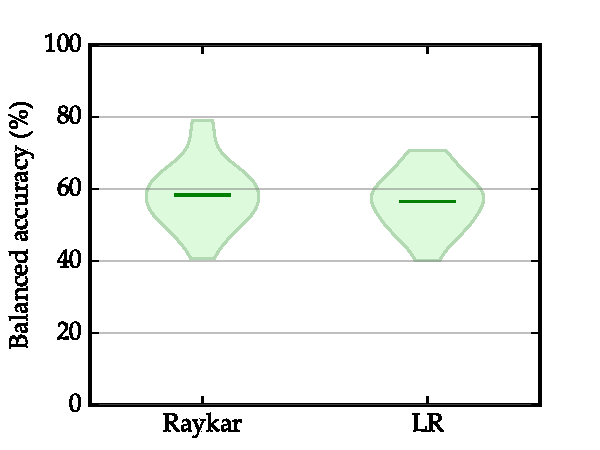
\includegraphics[width=\textwidth]{images/experiments/raykar.pdf}
                \caption{Performance of the \citeauthor{raykar10} classifier against logistic regression on a simulated crowd labelling of the breast cancer dataset \citep{wolberg90}.}
                \label{fig:raykar}
            \end{figure}

        \subsubsection{Yan et al. Method}

            \citet{yan10} propose modelling the $t$th labeller by a Bernoulli distribution of a data-dependent function $\eta_t(\vec x)$, parametrised as a logistic regression function $\eta_t(\vec x) = \sigma(\vec \omega_t^T \vec x + \gamma_t)$. The labeller model is thus
            \begin{equation*}
                p(y_t \mid \vec x, z, \vec \omega_t, \gamma_t) = \eta_t(\vec x)^{1 - |y_t - z|} (1 - \eta_t(\vec x))^{|y_t - z|}.
            \end{equation*}
            For ease of notation, let $\Omega = (\vec \omega_1^T, \dots, \vec \omega_T^T)$ and let $\vec \gamma = (\gamma_1, \dots, \gamma_T)$. This model can be obtained from the \citeauthor{raykar10} model by requiring $\alpha_t = \beta_t = \eta_t(\vec x)$ and allowing these parameters be data-dependent.

            As with \citeauthor{raykar10}, the classification model can be any classifier and \citeauthor{yan10} choose to use logistic regression (Equation \ref{eq:raykar-logreg}). The parameters $\vec \theta = \{\Omega, \vec \gamma, \vec w\}$ can be found by maximising the likelihood with expectation-maximisation. Under the assumptions that examples are independently sampled and that the labellers are independent, the likelihood is given by
            \begin{align*}
                p(\mathcal D \mid \vec \theta) &= \prod_{i = 1}^N \prod_{t = 1}^T p(y_{t, i} \mid \vec x_i, \vec w, \Omega, \vec \gamma)\\ &= \prod_{i = 1}^N \prod_{t = 1}^T \sum_{z = 0}^1 p(y_t \mid \vec x_i, z, \vec \omega_t, \gamma_t) p(z \mid \vec x_i, \vec w).
            \end{align*}
            The expectation steps requires us to compute
            \[
                \mu_i \propto \prod_{t = 1}^{T} p(y_{t, i} \mid \vec x_i, z_i = 1, \vec \omega_t, \gamma_t) p(z_i = 1 \mid \vec x_i, \vec w).
            \]
            The maximisation step requires us to maximise
            \begin{equation*}
                \sum_{i = 1}^N \sum_{t = 1}^T \sum_{z_i = 0}^1 p(z_i \mid \vec x_i, \vec w) (\log p(y_{t, i} \mid \vec x_i, z, \vec \omega_t, \gamma_t) + \log p(z \mid \vec x_i, \vec w))
            \end{equation*}
            with respect to $\vec w, \Omega,$ and $\vec \gamma$, where $p(z_i \mid \vec x_i, \vec w)$ is fixed to use the previous value of $\vec w$.